%! Tex program = xelatex   
\documentclass{homework}
\usepackage{xeCJK}
\usepackage{amsmath}
\usepackage{booktabs} %表格
% 
\setCJKmainfont{Kaiti SC}
% \setCJKfamilyfont{song}{Songti SC}
% \renewcommand{\baselinestretch}{1.5} %行间距
\author{朱浩泽 1911530}
\class{智能计算系统作业二}
\date{\today}
\title{\Large{智能计算系统二次作业}}

\graphicspath{{./media/}}

\begin{document} \maketitle

\question \large{以表3.7为例,计算置信度阈值为0.3时的精度(Precision)、召回率(Recall)、平均精度(AP)}

\normalsize
答:当置信度阈值为0.3时,我们认为第1、3、7、9、11、12、14、17、19、20为postive,但实际上只有第3、5、7、10、14、18、20为true positive,所以
\begin{align*}
	precision &= \frac{k}{N} = \frac{P}{TP+FP} = \frac{4}{4 + 6} = 0.4\\
	Recall &= \frac{k}{M} = \frac{TP}{TP+FN} = \frac{4}{25} = 0.16
\end{align*}
去掉置信度小于0.3的数据做下表:
\begin{center}
	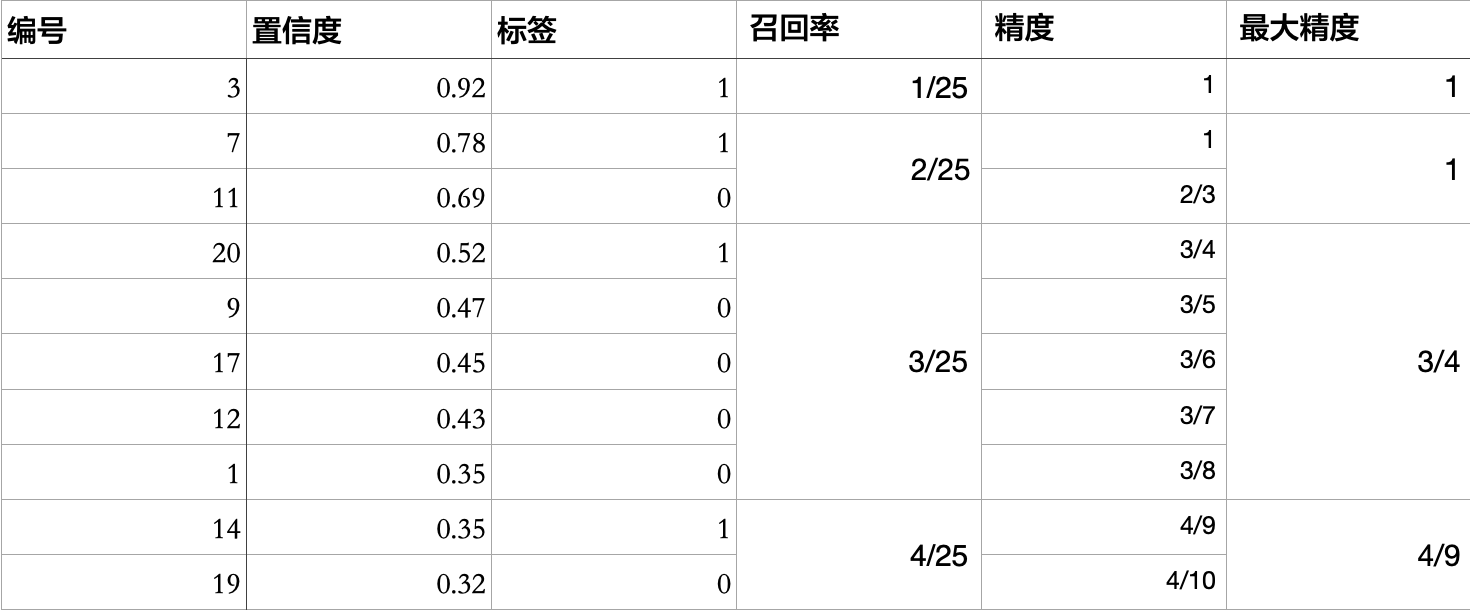
\includegraphics[scale = 0.5]{1.png}
\end{center}
$$
AP = \frac{(1 + 1 + 3/4 + 4/9)}{25}\approx 0.128 
$$
~\\ 
~\\
~\\ 
\question \large{通过比较已有的基于卷积神经网络的图像分类算法和图像目标检测算法,选取其中的某一方向谈一下对深度学习网络的认识;}

\normalsize
答:
\begin{itemize}
	\item \textbf{AlexNet} \\
	通过使用ReLU作为CNN的激活函数解决Sigmoid在网络较深时的梯度弥散问题\\ 
	通过在最后几个全连接层使用Dropout避免模型过拟合\\ 
	通过使用最大池化避免平均池化的模糊化效果,且步长比卷积核尺寸小\\ 
	通过LRN层使得响应大的值变得更大,并通过抑制反馈较小的值增强泛化能力\\ 
	通过随机从265*256的原始图像中截取224*224大小的区域进行数据增强以达到减轻过拟合、提升模型泛化能力的效果,并在预测时取图片的四个角和中间5个位置左右翻转,最后通过10次预测的结果求得平均值达到最终结果
	\item \textbf{VGG} \\ 
	反复堆叠3*3的小型卷积核和2*2的最大池化层,建立了16-19层的简洁结构\\
	拓展性强,迁移到其他图片数据上的泛化性非常好\\ 
	提供了非常好的初始化权重,经常被用来提取图像特征,可用于domain Specific 的图像分类任务上进行再训练\\ 
	多个小卷积层堆叠在一起,达到了利用更参数获得更大视野的目的,而且拥有更多的非线性变换,提高了学习能力\\ 
	在训练时先训练简单网络,后用简单网络的权重初始化复杂模型,加快收敛速度\\ 
	预测和训练采用了Multi-Scale方法对数据进行增强\\ 
	采用更深的神经网络以及更多的卷基层和非线性激活函数来提升分类准确率\\ 
	相对于AlexNet来说,参数更多但需要的迭代的次数更少
	\item \textbf{Inception} \\ 
	V1层层数相对较多,但参数却相对于AlexNet很少\\ 
	利用全局平均池化层取代最终的全连接层,使训练模型更快且减轻的过拟合\\ 
	提高了参数利用率和网络表达能力,同时可以对输出通道进行升维和降维,以达到利用很小的计算量便可以增加一层特征变换和非线性变换的目的\\ 
	在输出通道维度上通过聚合操作合并多个分支,增加了网络对不同尺寸的适应性\\ 
	通过一起发射的神经元连在一起这一特点达到学习过程中的刺激使神经元间的突触强度增强的目的
\end{itemize}
\par 通过上述三种主流基于卷积神经网络的图像分类算法和图像目标检测算法,可以看出目前主流的深度学习网络都会通过多层的神经网络进行正向传导和负向调节,并需要训练多轮次。但随之而来的问题是一个深度学习网络相邻各个层之间的各个神经元之间也需要大量的连接,导致参数的数目大量增长,这便需要需要利用大量的时间和算力,且过深的网络以及神经元之间的全连接以及过多的训练轮次可能会导致模型过拟合,所以现行的深度学习模型主要解决优化的就是这些方面的问题,以卷机神经网络为例,其主要思想便是通过局部连接大大减少网络的参数,并在卷积层中通过每个滤波器与上一层局部连接,同时每个滤波器的所有局部连接都使用同样的参数,来达到参数共享以控制参数的数量;并通过池化逐渐降低数据的空间尺寸,再次减少网络中参数的数量,使得计算资源耗费变少,也能有效控制过拟合。
~\\ 
~\\ 
~\\ 
\question \large{计算AlexNet、VGG19、ResNet152三个网络中神经元数目及可训练的参数数量,简述一下对于深度学习模型加速必要性的认识。}

\normalsize 
答:\begin{itemize}
	\item  \textbf{AlexNet} \\ 
	Input:224$\times$ 224$\times$ 3=150528\\ 
	CNN1: 96个11$\times$ 11$\times$ 3的卷积核,\\ 
	神经元数量为:55$\times$ 55$\times$ 48$\times$ 2=290400\\ 
	参数数量:11$\times$ 11$\times$ 3$\times$ 96+96=34944\\ 
	CNN2: 256个5$\times$ 5$\times$ 48卷积核,\\ 
	神经元数量为:27$\times$ 27$\times$ 128$\times$ 2=186624\\ 
	参数数量:(5$\times$ 5$\times$ 48$\times$ 128+128)$\times$ 2=307456\\ 
	CNN3: 384个3$\times$ 3$\times$ 256卷积核,\\ 
	神经元数量为:13$\times$ 13$\times$ 192$\times$ 2=64896\\ 
	参数数量:3$\times$ 3$\times$ 256$\times$ 384+384=885120\\ 
	CNN4: 384个3$\times$ 3$\times$ 192卷积核,\\ 
	神经元数量为:13$\times$ 13$\times$ 192$\times$ 2=64896\\ 
	参数数量:(3$\times$ 3$\times$ 192$\times$ 192+192)$\times$ 2=663936\\ 
	CNN5: 256个3$\times$ 3$\times$ 192卷积核,\\ 
	神经元数量为:13$\times$ 13$\times$ 128$\times$ 2=43264\\ 
	参数数量:(3$\times$ 3$\times$ 192$\times$ 128+128)$\times$ 2=442624\\ 
	FC1: \\ 
	神经元数量:4096\\ 
	参数数量:(6$\times$ 6$\times$ 128$\times$ 2)$\times$ 4096+4096=37752832\\ 
	FC2:\\  
	神经元数量:4096\\ 
	参数数量:4096$\times$ 4096+4096=16781312\\ 
	FC2: \\ 
	神经元数量:4096\\ 
	参数数量:4096$\times$ 1000+1000=4097000\\ 
	通过上面计算:
	神经元数量总数:809800\ \ \ \ \  
	参数数量总数:60965224
	\item \textbf{VGG19} \\ 
	同理,我们知道VGG19的结构是19层,同理上述计算可以算出神经元总数量为$64 + 64 + 128 + 128 + 256+256+256+256+512+512+512+512+512+512+512+512+4096+4096+1000 = 14696$个,参数总数为$3 \times 3 \times 3 \times 64 + 3 \times 3\times 64\times 64 +3\times  3\times 128+ 3\times 3\times 64\times 128+\cdots + 7\times 7\times 512 \times 4096+4096\times 4096+4096\times 1000 = 143652544$个
	\item \textbf{ResNet152}\\ 
	其网络结构和神经数目如下表,由于数值过于巨大,不再进行累加计算。
	\begin{center}
		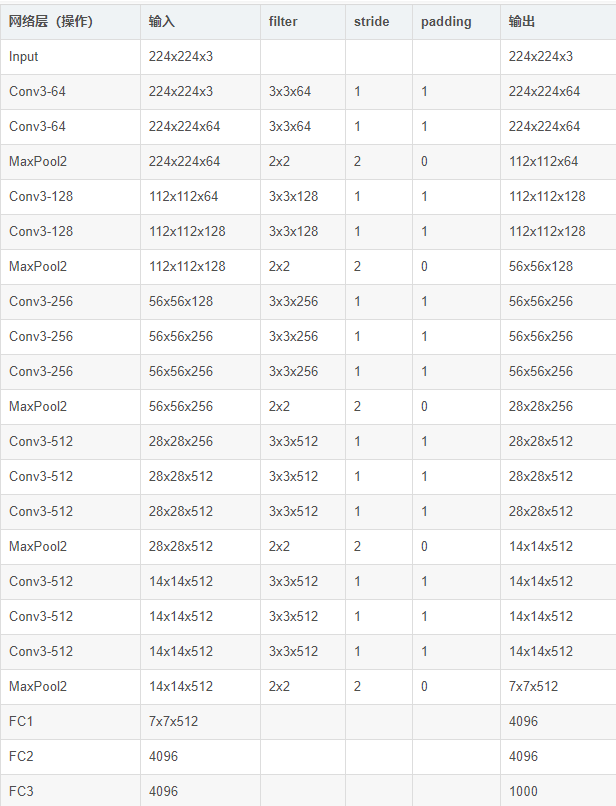
\includegraphics{CoeN3-64.png}
	\end{center}
	
\end{itemize}
~\\
通过以上计算,我们可以轻易的看出,深度学习模型的神经元和参数数量庞大,且要经历多轮次的向前传递和负向反馈过程,每次都需要对每个参数进行更新,所以对于这种庞大的计算量,深度学习模型的加速就显得尤为重要。

\end{document}